\documentclass{article}
\usepackage{graphicx}
\usepackage{amsmath}
\usepackage{enumitem}
\usepackage{float}
\usepackage{listings}
\usepackage{AMP-report-style}
\usepackage{xcolor}
\usepackage[a4paper, margin=1in]{geometry}
\title{Project \\ \large Quadcopter Drone Kinodynamical Motion Planning}
\author{Steve Gillet}
\date{\today}

% Custom information
\newcommand{\className}{Course: Algorithmic Motion Planning – ASEN 5254-001 – Fall 2024}
\newcommand{\professorName}{Professor: Morteza Lahijanian}
\newcommand{\taName}{Teaching Assistant: Yusif Razzaq}

\lstdefinestyle{cppstyle}{
    language=C++,                 % Specify the language
    basicstyle=\ttfamily\footnotesize\color{black}, % Code font
    keywordstyle=\color{red}\bfseries, % Keywords
    stringstyle=\color{red},      % Strings
    commentstyle=\color{red},    % Comments
    numbers=left,                 % Line numbers
    numberstyle=\tiny\color{black},% Line number style
    stepnumber=1,                 % Line number increment
    breaklines=true,              % Line breaking
    frame=single,                 % Border around code
    backgroundcolor=\color{white},
    tabsize=4,                    % Tab size
    showstringspaces=false,       % Don't show spaces in strings
}

\begin{document}

\maketitle

\section*{Overview}
The goal of this project is to take the dynamics for a quadcopter that I developed in another class (Linear Control Systems) and use them to develop kinodynamical motion planning for a quadcopter.
I will have to add kinodymical constraints and probably adapt the dynamics that I already have in other ways to make them fit the problem here.
I think the ultimate plan is to be able to come up with something like a delivery plan for a quadcopter dropping off packages from a delivery truck or some similar problem with multiple waypoints.

\section*{Starting Dynamics}

These are the dynamics that I used and developed in Linear Control Systems.

\subsection*{Introduction}

Multirotors are versatile vehicles with a wide variety of applications. They also represent an inter-
esting control problem as they are inherently unstable. The vehicle is controlled by commands that
alter the trust produced by the rotors.

\subsection*{Physical System}
  
\begin{figure}[H]    
    \centering
    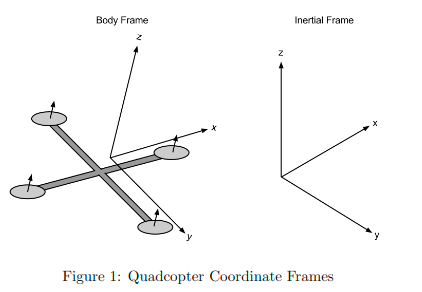
\includegraphics[width=0.6\linewidth]{quadcopterFrameFigure.png}
\end{figure}

\subsection*{Linearized State Space Model}

Assuming a symmetric vehicle with four identical rotors, where one pair spins in one direction and
the other pair spins in the opposite direction, the following linearized model can be derived for
motion in the neighborhood of level hovering flight.

State variables in this model are
$x = \begin{bmatrix} x & \dot{x} & y & \dot{y} & z & \dot{z} \end{bmatrix}$
consisting of inertial positions and velocities in the X, Y , and Z directions. It is assumed that an
inner loop control is acting to keep the vehicle in a horizontal orientation, and to keep the body
x axis pointing in the X direction. It also assumed that the rotor normals are all tilted in toward
the center of the vehicle at a fixed angle, so that a component of the thrust in each is available for
horizontal translation. There are four rotor thrust controls (inputs) T1 through T4. These produce
perturbation forces (away from the nominal needed to oppose the vehicle\'s weight) as follows.

\begin{align*}
    F_X &= \delta(T_3 - T_1) \\
    F_Y &= \delta(T_4 - T_2) \\
    F_Z &= \gamma(T_1 + T_2 + T_3 + T_4)
\end{align*}
     
The motion of the vehicle is retarded by aerodynamic drag, using the $k_{d,lat}$ and $k_{d,vert}$ coefficients
in units of $[ \frac{N \cdot s}{m} ]$. Vehicle mass is given by m. Outputs are the X, Y , and Z positions, given by
GPS.

The resulting state space realization

$\dot{x} = Ax + Bu$

$y = Cx + Du$

has the specific form:

\[
A = 
\begin{bmatrix}
0 & 1 & 0 & 0 & 0 & 0 \\
0 & -\frac{k_{d,lat}}{m} & 0 & 0 & 0 & 0 \\
0 & 0 & 0 & 1 & 0 & 0 \\
0 & 0 & 0 & -\frac{k_{d,lat}}{m} & 0 & 0 \\
0 & 0 & 0 & 0 & 0 & 1 \\
0 & 0 & 0 & 0 & 0 & -\frac{k_{d,vert}}{m} \\
\end{bmatrix}
\]

\[
B = 
\begin{bmatrix}
0 & 0 & 0 & 0 \\
-\frac{\delta}{m} & 0 & \frac{\delta}{m} & 0 \\
0 & 0 & 0 & 0 \\
0 & -\frac{\delta}{m} & 0 & \frac{\delta}{m} \\
0 & 0 & 0 & 0 \\
\frac{\gamma}{m} & \frac{\gamma}{m} & \frac{\gamma}{m} & \frac{\gamma}{m} \\
\end{bmatrix}
\]

\[
u = 
\begin{bmatrix}
T_1 \\
T_2 \\
T_3 \\
T_4 \\
\end{bmatrix}
\]

Using parameters from a particular vehicle, we get the following values for the state-space realization:

\[
\dot{x} = 
\begin{bmatrix}
0 & 1 & 0 & 0 & 0 & 0 \\
0 & -0.0104 & 0 & 0 & 0 & 0 \\
0 & 0 & 0 & 1 & 0 & 0 \\
0 & 0 & 0 & -0.0104 & 0 & 0 \\
0 & 0 & 0 & 0 & 0 & 1 \\
0 & 0 & 0 & 0 & 0 & -0.0208 \\
\end{bmatrix}
x +
\begin{bmatrix}
0 & 0 & 0 & 0 \\
-0.04167 & 0 & 0.04167 & 0 \\
0 & 0 & 0 & 0 \\
0 & -0.04167 & 0 & 0.04167 \\
0 & 0 & 0 & 0 \\
0.4 & 0.4 & 0.4 & 0.4 \\
\end{bmatrix}
u
\]

\[
y = 
\begin{bmatrix}
1 & 0 & 0 & 0 & 0 & 0 \\
0 & 0 & 1 & 0 & 0 & 0 \\
0 & 0 & 0 & 0 & 1 & 0 \\
\end{bmatrix}
x +
\begin{bmatrix}
0 & 0 & 0 & 0 \\
0 & 0 & 0 & 0 \\
0 & 0 & 0 & 0 \\
\end{bmatrix}
u
\]

\section*{3D Motion Planning}

I've decided to start off by adapting the 2-dimensional RRT motion planning that I developed for one of the class assignments to 3 dimensions.
The initial challenege is to just create a structure that I can use to develop, test, and visualize my motion plan since the toolbox structure that I used before will be difficult or impossible to adapt and has unnecessary componenents.
I started off by copying over my RRT implementation and then building out the pieces of it that had been provided by the toolbox previously.
This includes structures like Path2D, Problem2D, and Node which all of course had to be adapted to 3 dimensions.
It turns out that a lot of what Graph and Path were doing were superfluous and I didn't really need for my simple implementation so I threw out.

I created Node as a simple structure with x, y, z, an id number, and a children vector so the children can be kept track of when it comes time to do a graph search to find the best path.
I created Obstacle as another simple structure with a vector of vertices and the Problem structure keeps a vector pair of id numbers with obstacles so I can keep track of which obstacle is which when visualizing.
I had to create a new function to check for collisions in 3 dimensions so I started with this overly simplified pointInPolyhedron function that checks if a point is within the min and max vertex in a set of vertices.
This of course is not actually a sufficient method for anything except an axis-aligned cube, but I have the concept for a more thorough check that I will discuss later.

I also created a Problem3D struct which has the basics of the Problem classes that we used in class.
It has workspace boundaries, a starting and goal points, and the vector of obstacles.
I also copied over my aStar implementation and simplified it to just a success bool, path, and path length variables as well as a search method.
As far as the implementation goes it basically stayed the same except that the RRT function now operates in 3 dimensions and returns an aStar object.
The A* implementation was simplified to not use Graph or Path anymore and just keep a couple of vectors of Nodes and a vector of back pointers.
The children for the Nodes are set in the RRT algorithm and whenever the lowest cost node is updated, the back pointer is updated.

Lastly, I had to define the obstacles now in the main section as a set of vertices and then create some functions to save the obstacles and path to csv files for the visualizer to use.
The visualizer is a relatively simple Python script which uses matplotlib toolkits to visualize 3D Polyhedrons for the obstacles and plots everything on a 3D scatter plot.
You can see my implementation in the code section below.

\subsection*{Include File}
\begin{lstlisting}[style=cppstyle]
#include <Eigen/Core>
#include <vector>

struct Node {
    int id;
    double x;
    double y;
    double z;
    std::vector<int> children;

    Node(int idIn, double xIn, double yIn, double zIn, std::vector<int> childrenIn){
        id = idIn;
        x = xIn;
        y = yIn;
        z = zIn;
        children = childrenIn;
    }
};

struct Obstacle3D{
    std::vector<Eigen::Vector3d> vertices;

    Obstacle3D(std::vector<Eigen::Vector3d> verticesIn){
        vertices = verticesIn;
    }
};

bool isPointInPolyhedron(std::vector<Eigen::Vector3d> vertices, Eigen::Vector3d point);

struct Problem3D{
    Eigen::Vector3d qInit;
    Eigen::Vector3d qGoal;
    std::vector<std::pair<int, Obstacle3D>> obstacles;
    double xMin, xMax;
    double yMin, yMax;
    double zMin, zMax;

    Problem3D(Eigen::Vector3d qInitIn, Eigen::Vector3d qGoalIn, std::vector<std::pair<int, Obstacle3D>> obstaclesIn, double xMinIn, double xMaxIn, double yMinIn, double yMaxIn, double zMinIn, double zMaxIn){
        qInit = qInitIn;
        qGoal = qGoalIn;
        obstacles = obstaclesIn;
        xMin = xMinIn;
        xMax = xMaxIn;
        yMin = yMinIn;
        yMax = yMaxIn;
        zMin = zMinIn;
        zMax = zMaxIn;
    }
};

double heuristic(Node node, Eigen::Vector3d goal);

class aStar{
public:
    bool success;
    std::vector<Node> path; 
    double pathCost;

    aStar(bool successIn, std::vector<Node> pathIn, double pathCostIn){
        success = successIn;
        path = pathIn;
        pathCost = pathCostIn;
    }

    void search(Problem3D problem, std::vector<Node> nodes);
};

aStar rrt(const Problem3D& problem, int n, double r, double epsilon, double p);
\end{lstlisting}

\subsection*{Source File}
\begin{lstlisting}[style=cppstyle]
#include "rrt.h"
#include <cmath>
#include <random>
#include <iostream>

bool isPointInPolyhedron(std::vector<Eigen::Vector3d> vertices, Eigen::Vector3d point){
    Eigen::Vector3d min = vertices[0];
    Eigen::Vector3d max = vertices[0];

    for (const auto& vertex : vertices) {
        min = min.cwiseMin(vertex);
        max = max.cwiseMax(vertex);
    }

    return (point.x() >= min.x() && point.x() <= max.x() &&
            point.y() >= min.y() && point.y() <= max.y() &&
            point.z() >= min.z() && point.z() <= max.z());
}

double heuristic(Node node, Eigen::Vector3d goal){
    return std::sqrt(
        std::pow(goal.x() - node.x, 2) +
        std::pow(goal.y() - node.y, 2) +
        std::pow(goal.z() - node.z, 2) 
    );
}

void aStar::search(Problem3D problem, std::vector<Node> nodes){
    std::vector<Node> openList;
    std::vector<Node> closedList;
    std::vector<double> gCost(nodes.size(), __DBL_MAX__);
    std::vector<double> fCost(nodes.size(), __DBL_MAX__);
    std::vector<int> backPointer(nodes.size(), -1);
    int startId = nodes[0].id;
    int goalId = nodes[nodes.size() - 1].id;

    Node& startNode = nodes[0];
    openList.push_back(startNode);
    gCost[startId] = 0.0;
    fCost[startId] = gCost[startId] + heuristic(startNode, problem.qGoal);
    backPointer[startId] = startId;

    while (!openList.empty()){
        Node current(-1, 0.0, 0.0, 0.0, {});
        double minCost = __DBL_MAX__;
        for(Node& item : openList){
            if(fCost[item.id] < minCost){
                minCost = fCost[item.id];
                current = item;
            }
        }
        
        auto it = std::find_if(openList.begin(), openList.end(), [&](Node& n) {
            return n.id == current.id;
        });
        openList.erase(it);
        closedList.push_back(current);
        
        if(current.id == goalId){
            this->success = true;
            this->pathCost = gCost[current.id];
            this->path.push_back(nodes[current.id]);

            int it = current.id;
            while(it != startId){
                this->path.push_back(nodes[backPointer[it]]);
                it = backPointer[it];
            }

            std::reverse(this->path.begin(), this->path.end());
            return;
        }

        for(int childIndex : current.children){
            Node& child = nodes[childIndex];
            bool childInClosedList = false;
            for(Node& compare : closedList){
                if(child.id == compare.id) childInClosedList = true;
            }
            if(!childInClosedList){
                bool childInOpenList = false;
                for(Node& compare : openList){
                    if(child.id == compare.id) childInOpenList = true;
                }

                double potentialG = gCost[current.id] + heuristic(current, Eigen::Vector3d(child.x, child.y, child.z));
                if(!childInOpenList){
                    openList.push_back(child);
                    backPointer[child.id] = current.id;
                    gCost[child.id] = potentialG;
                    fCost[child.id] = potentialG + heuristic(child, problem.qGoal); 
                } 
                else if (potentialG < gCost[child.id])
                {
                    backPointer[child.id] = current.id;
                    gCost[child.id] = potentialG;
                    fCost[child.id] = potentialG + heuristic(child, problem.qGoal);  
                }
            }
        }
    }
}

aStar rrt(const Problem3D& problem, int n, double r, double epsilon, double p){
    static std::random_device rd;
    static std::mt19937 gen(rd());

    std::vector<Node> nodes;
    nodes.emplace_back(Node(0, problem.qInit.x(), problem.qInit.y(), problem.qInit.z(), {}));
    int currentNodeIndex = 1;

    int counter = 0;
    bool pathFound = false;

    while (counter < n && !pathFound) {
        Eigen::Vector3d point;
        std::bernoulli_distribution bernoulli(p);

        if (bernoulli(gen)) {
            point = problem.qGoal; // Biased towards the goal
        } else {
            std::uniform_real_distribution<> xdis(problem.xMin, problem.xMax);
            std::uniform_real_distribution<> ydis(problem.yMin, problem.yMax);
            std::uniform_real_distribution<> zdis(problem.zMin, problem.zMax);
            point = Eigen::Vector3d(xdis(gen), ydis(gen), zdis(gen));
        }

        double distance = __DBL_MAX__;
        int qNearIndex = 0;
        for(int i = 0; i < nodes.size(); i++){
            double currentDistance = (point - Eigen::Vector3d(nodes[i].x, nodes[i].y, nodes[i].z)).norm();
            if(distance > currentDistance){
                qNearIndex = i;
                distance = currentDistance;
            } 
        }

        Eigen::Vector3d qNear = Eigen::Vector3d(nodes[qNearIndex].x, nodes[qNearIndex].y, nodes[qNearIndex].z);
        Eigen::Vector3d step = r * (point - qNear).normalized();
        Eigen::Vector3d qNew = qNear + step;

        bool pointInObstacle = false;
        for (auto& obstacle : problem.obstacles) {
            if (isPointInPolyhedron(obstacle.second.vertices, qNew)){
                pointInObstacle = true;
                break;
            } 
        }

        if(!pointInObstacle){
            nodes.emplace_back(Node(currentNodeIndex, qNew.x(), qNew.y(), qNew.z(), {}));
            currentNodeIndex++;
            nodes[qNearIndex].children.push_back(currentNodeIndex);

            if ((qNew - problem.qGoal).norm() < epsilon) {
                pathFound = true;
                nodes.emplace_back(Node(currentNodeIndex, problem.qGoal.x(), problem.qGoal.y(), problem.qGoal.z(), {}));
            }

        }
        counter++;
    }

    aStar astar(false, {}, 0.0);

    if(!pathFound){
        std::cout << "Path not found in rrt." << std::endl;
        return astar;
    }

    astar.search(problem, nodes);
    return astar;
}
\end{lstlisting}

\subsection*{Main File}
\begin{lstlisting}[style=cppstyle]
#include "rrt.h"
#include <fstream>
#include <iostream>


void exportPathToCSV(std::vector<Node> path, std::string fileName){
    std::ofstream file(fileName);
    if (!file.is_open()){
        std::cerr << "Failed to open file for writing: " << fileName << std::endl;
        return;
    }

    file << "x,y,z\n";
    for (auto waypoint : path){
        file << waypoint.x << "," << waypoint.y << "," << waypoint.z << "\n";
    }

    file.close();
}

void exportObstaclesToCSV(std::vector<std::pair<int, Obstacle3D>> obstacles, std::string fileName){
    std::ofstream file(fileName);
    if (!file.is_open()){
        std::cerr << "Failed to open file for writing: " << fileName << std::endl;
        return;
    }

    file << "id,x,y,z\n";
    for (auto obstacle : obstacles){
        int id = obstacle.first;
        for (auto vertex : obstacle.second.vertices){
            file << id << "," << vertex.x() << "," << vertex.y() << "," << vertex.z() << "\n";
        }
    }
    file.close();
    std::cout << "Obstacles written to " << fileName << std::endl;
}

int main(){
    // Define obstacles
    std::vector<std::pair<int, Obstacle3D>> obstacles;
    obstacles.emplace_back(1, std::vector<Eigen::Vector3d>{
        Eigen::Vector3d(2.0, 2.0, 2.0),
        Eigen::Vector3d(4.0, 2.0, 2.0),
        Eigen::Vector3d(4.0, 4.0, 2.0),
        Eigen::Vector3d(2.0, 4.0, 2.0),
        Eigen::Vector3d(2.0, 2.0, 4.0)
    });
    obstacles.emplace_back(2, std::vector<Eigen::Vector3d>{
        Eigen::Vector3d(8.0, 8.0, 8.0),
        Eigen::Vector3d(8.0, 8.0, 6.0),
        Eigen::Vector3d(8.0, 6.0, 8.0),
        Eigen::Vector3d(8.0, 6.0, 6.0),
        Eigen::Vector3d(10.0, 8.0, 8.0),
        Eigen::Vector3d(10.0, 8.0, 6.0),
        Eigen::Vector3d(10.0, 6.0, 8.0),
        Eigen::Vector3d(10.0, 6.0, 6.0)
    });

    // Define bounds
    double xMin = 0.0, xMax = 15.0;
    double yMin = 0.0, yMax = 15.0;
    double zMin = 0.0, zMax = 15.0;

    Eigen::Vector3d qInit(0.0, 0.0, 0.0);  // Start position
    Eigen::Vector3d qGoal(10.0, 10.0, 10.0);  // Goal position
    // Create the 3D motion planning problem
    Problem3D problem(qInit, qGoal, obstacles, xMin, xMax, yMin, yMax, zMin, zMax);

    int n = 1000;
    // step size
    double r = 1.0;
    double epsilon = 0.5; // Goal Radius
    double p = 0.05; // Goal Bias

    aStar astar(false, {}, 0.0);
    astar = rrt(problem, n, r, epsilon, p);

    if (astar.success){
        std::cout << "Path found!" << std::endl;
        std::cout << "Path length: " << astar.pathCost << std::endl;

        exportPathToCSV(astar.path, "path.csv");
        exportObstaclesToCSV(problem.obstacles, "obstacles.csv");
    } else{
        std::cout << "No path found." << std::endl;
    }

    return 0;
}
\end{lstlisting}

\subsection*{Lessons Learned}

My initial simplified implementation was successful as you can see in the image below.

\begin{figure}[H]
    \centering
    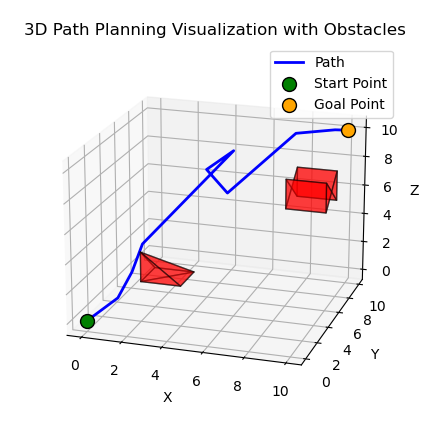
\includegraphics[width=0.7\linewidth]{3DrrtPlot.png}
\end{figure}

The way I am plotting the obstacles currently means that I am looking for specific shapes and plotting the faces in a specific order by the order of the vertices which gives some weird looking obstacle plots.
My plan for improving that is to just go through each obstacle and plot every three vertices as a face and hopefully that will have a more consistent look to it.

I also plan to implement an expansion of the obstacles to keep the paths a bit further away from them because they cut a bit close sometimes and that will be helpful for the kinodynamics anyways.
Most importantly I want to improve my obstacle detection and my plan for that is to implement a checker function that checks if a line intersects a face.
This will have the dual purpose as serving as the basis of ray casting and for path smoothing.
Ray casting is when you take a point and you randomly shoot out a line from that point and count the number of face intersections for a particular object with that line and if the number of intersections is even (including 0) then the point is not in the object and if it is odd then it is.
For path smoothing I will be able to check if the line between any vertices intersects the face of any obstacle before using that line as the new shorter path.

\section*{3D Collision Detection}

\subsection*{Line in Face}

I implemented a function to check if a 3-dimensional line intersects a 2-dimensional bounded plane in a 3-dimensional space (henceforth referred to as a face).
I started with using the equations of planes and lines to find where the intersection point is.
Parametric equation for line:

\begin{align*}
    P(t) = P_0 + td
\end{align*}

Where $P_0$ is a point on the line, d is the direction vector, and t is a scalar.
Equation for plane:

\begin{align*}
    n \cdot (x - p_0) = 0 
\end{align*}

Where n is the normal vector and x and $p_0$ are points on the plane.
Putting these equations together and solving for t you can get where the line segment intersects the plane.

\begin{align*}
    t = \frac{-n \cdot (P_0 - p_0)}{n \cdot d}
\end{align*}

If t is between 0 and 1 then the intersection point is within the line segment bounds.
Next I used Barycentric Coordinates to test if the point is within the face.
In order to make this work I had to break the face up into triangles, so I basically just iterated through all of the vertices of the face and took three of them at a time.
Barycentric Coordinates essentially work by expressing a point as a linear combination of the three vertices of a triangle and if the linear combination scalars are all between 0 and 1 then the point lies inside the triangle indicating that none of the vectors have to be scaled outside the bounds of the triangle.
The equation looks like this:

\begin{align*}
    P = uA + vB + wC \quad with \quad u + v + w = 1
\end{align*}

You calculate u, v, and w by defining vectors between the vertices and point and calculating the area of the triangles those vectors form.
Let $v_0 = A$, $v_1 = B$, and $v_2 = C$.

\begin{align*}
    v_{10} &= v_1 - v_0 \\
    v_{20} &= v_2 - v_0 \\
    v_{P0} &= P - v_0
\end{align*}

Finding the area of $\Delta{PBC}$ gives you u.

\begin{align*}
    u = \frac{\|v_{P0} \times v_{20}\|}{\|v_{10} \times v_{20}\|}
\end{align*}

Similarly, $\Delta{APC}$ gives v.

\begin{align*}
    v = \frac{\|v_{10} \times v_{P0}\|}{\|v_{10} \times v_{20}\|}
\end{align*}

And you can get w from u and v:

\begin{align*}
    w = 1 - u - v
\end{align*}

My implementation in C++ code is shown below:

\begin{lstlisting}[style=cppstyle]
bool isLineInFace(std::vector<Eigen::Vector3d> faceVertices, std::vector<Eigen::Vector3d> lineVertices){
    Eigen::Vector3d lineDirection = lineVertices[1] - lineVertices[0];
    for (int i = 0; i < faceVertices.size(); i++) {
        Eigen::Vector3d A = faceVertices[i];
        Eigen::Vector3d B = faceVertices[(i+1)%faceVertices.size()];
        Eigen::Vector3d C = faceVertices[(i+2)%faceVertices.size()];

        Eigen::Vector3d normal = (B-A).cross(C-A).normalized();

        double denom = normal.dot(lineDirection);
        double t = -1.0;
        if (std::abs(denom) > 1e-8){
            t = -normal.dot(lineVertices[0] - A) / denom;
        }

        if (t >= 0 && t <= 1){
            Eigen::Vector3d intersectionPoint = lineVertices[0] + (lineVertices[1] - lineVertices[0]) * t;
            Eigen::Vector3d v0 = C - A;
            Eigen::Vector3d v1 = B - A;
            Eigen::Vector3d v2 = intersectionPoint - A;

            double dot00 = v0.dot(v0);
            double dot01 = v0.dot(v1);
            double dot02 = v0.dot(v2);
            double dot11 = v1.dot(v1);
            double dot12 = v1.dot(v2);

            double invDenom = 1 / (dot00 * dot11 - dot01 * dot01);
            double u = (dot11 * dot02 - dot01 * dot12) * invDenom;
            double v = (dot00 * dot12 - dot01 * dot02) * invDenom;

            if ((u >= 0) && (v >= 0) && (u + v < 1)) return true;
        }
    }
    return false;
}
\end{lstlisting}

\subsection*{Path Smoothing}

This allowed me to change the way I was checking for obstacles to be a bit more thorough.
Now I am able to just cycle through the faces of each obstacle and determine if my path intersects any of them.
This also allowed me to implement path smoothing because I could now check an entire path segment for collisions.
Allowing me to check if any intermediary paths between any two points is legitimate.
I implemented it using code I had developed earlier which simply chooses any two random points on your path and checks if a new path can be drawn in between them.

You can see the results in the plots below where I took the same 3D RRT path before and after smoothing.
You can see how the smoothed path is the same minus a couple of points.

\begin{figure}[H]
    \centering
    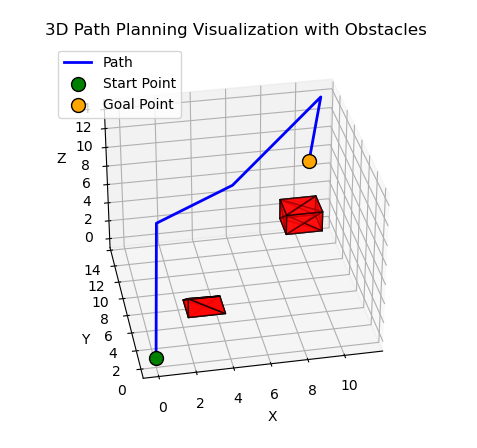
\includegraphics[width=0.49\linewidth]{preSmoothPath.png}
    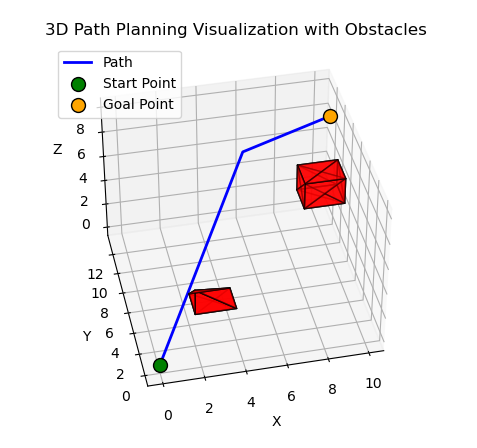
\includegraphics[width=0.49\linewidth]{postSmoothPath.png}
\end{figure}

My implementation is shown below:

\begin{lstlisting}[style=cppstyle]
void smoothPath(aStar& astar, Problem3D& problem) {
    const int maxIterations = 50;  // Number of smoothing attempts

    for (int j = 0; j < maxIterations; j++) {
        // Randomly pick two waypoints in the path
        if (astar.path.size() <= 2) {
            break;  // No smoothing needed for fewer than 3 waypoints
        }

        int index1 = std::rand() % astar.path.size();
        int index2 = std::rand() % astar.path.size();

        // Ensure index1 < index2
        if (index1 > index2) std::swap(index1, index2);
        if (index2 - index1 <= 1) continue;  // Skip consecutive points

        Eigen::Vector3d p1(astar.path[index1].x, astar.path[index1].y, astar.path[index1].z);
        Eigen::Vector3d p2(astar.path[index2].x, astar.path[index2].y, astar.path[index2].z);

        bool collisionFree = true;
        for (auto obstacle : problem.obstacles) {
            for (auto& face : obstacle.second.faces){
                if (isLineInFace(face, {p1, p2})){
                    collisionFree = false;
                    break;
                } 
            }
            if (!collisionFree) break;
        }

        // If the straight line is valid, remove the intermediate waypoints
        if (collisionFree) {
            astar.path.erase(astar.path.begin() + index1 + 1, astar.path.begin() + index2);
        }
    }
}
\end{lstlisting}

\section*{Kinodynamics}

I started out by coming up with a basic kinodynamic framework using some of the dynamics from the first section plus some constraints that I came up with using research and simplified numbers to start out with.
So the state space of the drone include the position in x, y, z coordinates and is constrained by the arbitrary boundaries that I had originally set up for my workspace (0 to 15 for each dimension).
As well as the x, y, and z velocities which are constrained by plus and minus 20 meters per second which is somewhere around the average max velocity for a consumer drone.
The controls I simplified to x, y, and z force which are limited to 100 Newtons and -50 Newtons again based on average consumer products.

I then created a new RRT function for the state space based on the kinodynamical RRT I created for the kinodynamic homework assignment adapted to the new structure and expanded to the new state space.
This involves basically the same logic as before except that the randomly sampled point is sampled across the whole state space and a random duration is genered.
A control must also be generated to actually take the drone from the nearest node to the sample node, which I generated by using the velocity components of the sampled and nearest nodes and Newton's formula for force, F=ma.

\begin{align*}
    F_x &= m \cdot \frac{\Delta v_x}{\Delta t}, \\
    F_y &= m \cdot \frac{\Delta v_y}{\Delta t}, \\
    F_z &= m \cdot \frac{\Delta v_z}{\Delta t} + m \cdot g
\end{align*}

I simplified the mass of the drone and gravity here to 2kg and $9.8m/s^2$.
Then I added a check to see if the controls were in bounds as well as the states and if the path passes through an obstacle.
I also had to change the A* search function to accomodate the new node structure since the state nodes now had state vectors instead of just x, y, z.
And I had to enhance the path smoothing function since the controls that take the drone on a new trajectory also have to be within bounds.
I also had Grok generate a fun little Python script to animate the drone moving through the path at different velocities using the 'FuncAnimation' library from matplotlib:

\begin{figure}[H]
    \centering
    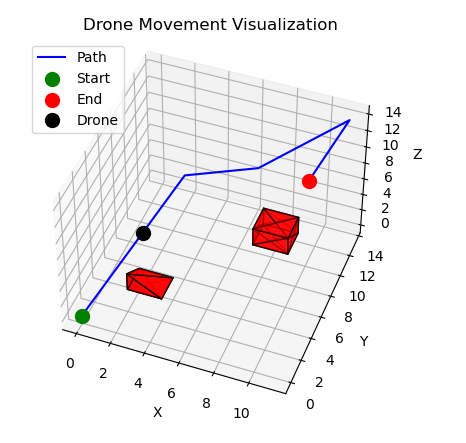
\includegraphics[width=0.7\linewidth]{kinoAnimation.png}
\end{figure}

I noticed that I had possibly created an issue because I was no longer taking steps towards the sampled state that if the sampled state was reachable within the control parameters that the path might take quite large steps like you can see in that image in the first step there it goes all the way across the workspace and if these steps are too big then that might introduce some more room for error when it comes to more complicated kinodynamics, but also that's only 15 meters so maybe in the world of drones that's actually not that big of a problem.
Either way, something to keep an eye on.

My implementation for the kinodynamic modifications:

\begin{lstlisting}[style=cppstyle]
aStar kinoRRT(Problem3D& problem, kinoAgent& agent, int& n, double& epsilon, double& p) {
    int uSamples = 15;
    double m = 2.0;
    double g = 9.8;
    static std::random_device rd;
    static std::mt19937 gen(rd());
    int numStates = agent.states.size();
    
    std::vector<stateNode> nodes;
    std::vector<Eigen::VectorXd> points;
    std::map<std::pair<int, int>, Eigen::VectorXd> storedControls;
    std::map<std::pair<int, int>, double> storedDurations;

    points.push_back(problem.qInit);
    Eigen::VectorXd initialState(6);
    initialState << problem.qInit.x(), problem.qInit.y(), problem.qInit.z(), 0.0, 0.0, 0.0;
    nodes.emplace_back(stateNode(0, initialState, {}));
    int currentNodeIndex = 1;

    // Sampling random points
    int counter = 0;
    bool pathFound = false;
    while (counter < n && !pathFound) {
        Eigen::VectorXd point(numStates);
        std::bernoulli_distribution bernoulli(p);

        if(bernoulli(gen)){
            point = (Eigen::VectorXd(6) << problem.qGoal.x(), problem.qGoal.y(), problem.qGoal.z(), 0.0, 0.0, 0.0).finished();
        }
        else{
            for (int i = 0; i < agent.states.size(); i++) {
                double lower = agent.stateLowerBounds[i];
                double upper = agent.stateUpperBounds[i];
                std::uniform_real_distribution<> dis(lower, upper);
                point[i] = dis(gen);
            }
        }
        std::uniform_real_distribution<> randomDT(0.1, 1);
        double dt = randomDT(gen);

        Eigen::VectorXd qNear = nodes[0].state;
        double distance = __DBL_MAX__;
        int qNearIndex = 0;
        for(int i = 0; i < nodes.size(); i++){
            double currentDistance = (point - nodes[i].state).norm();
            if(distance > currentDistance){
                qNear = nodes[i].state;
                qNearIndex = i;
                distance = currentDistance;
            } 
        }

        Eigen::VectorXd potentialControl(3);
        potentialControl << m*(point[3] - qNear[3])/dt, m*(point[4] - qNear[4])/dt, m*(point[5] - qNear[5])/dt + m*g;
        bool controlInBounds = true;

        for (int i = 0; i < agent.controlLowerBounds.size(); i++){
            if (potentialControl[i] < agent.controlLowerBounds[i]) controlInBounds = false;
        }
        for (int i = 0; i < agent.controlUpperBounds.size(); i++){
            if (potentialControl[i] > agent.controlUpperBounds[i]) controlInBounds = false;
        }
        // std::vector<double> potentialDts;

        bool pathInObstacle = false;

        for (auto obstacle : problem.obstacles) {
            for (auto& face : obstacle.second.faces){
                if (isLineInFace(face, {{qNear[0], qNear[1], qNear[2]}, {point[0], point[1], point[2]}})){
                    pathInObstacle = true;
                    break;
                } 
            }
            if (pathInObstacle) break;
        }

        if (controlInBounds && !pathInObstacle){
            nodes.emplace_back(stateNode(currentNodeIndex, point, {}));
            nodes[qNearIndex].children.push_back(currentNodeIndex);

            storedControls[{qNearIndex, currentNodeIndex}] = potentialControl;
            storedDurations[{qNearIndex, currentNodeIndex}] = dt;
            if ((Eigen::Vector3d(point[0], point[1], point[2]) - problem.qGoal).norm() < epsilon) {
                pathFound = true;
            }

            currentNodeIndex++;
        }
            

        counter++;
    }

    std::vector<stateNode> empty;
    aStar astar(false, empty, 0.0);

    if(!pathFound){
        std::cout << "Path not found in rrt." << std::endl;
        return astar;
    }

    astar.searchState(problem, nodes);
    
    return astar;
}

void smoothStatePath(aStar& astar, Problem3D& problem, kinoAgent& agent) {
    const int maxIterations = 100;  // Number of smoothing attempts
    static std::random_device rd;
    static std::mt19937 gen(rd());
    double m = 2.0;
    double g = 9.8;
    // bool smoothingFound = false;


    for (int j = 0; j < maxIterations; j++) {
        // Randomly pick two waypoints in the path

        if (astar.statePath.size() <= 2) {
            break;  // No smoothing needed for fewer than 3 waypoints
        }

        int index1 = std::rand() % astar.statePath.size();
        int index2 = std::rand() % astar.statePath.size();

        // Ensure index1 < index2
        if (index1 > index2) std::swap(index1, index2);
        if (index2 - index1 <= 1) continue;  // Skip consecutive points

        Eigen::VectorXd p1(6);
        p1 = astar.statePath[index1].state;
        Eigen::VectorXd p2(6);
        p2 = astar.statePath[index2].state;

        bool collisionFree = true;
        for (auto obstacle : problem.obstacles) {
            for (auto& face : obstacle.second.faces){
                if (isLineInFace(face, {Eigen::Vector3d(p1[0], p1[1], p1[2]), Eigen::Vector3d(p2[0], p2[1], p2[2])})){
                    collisionFree = false;
                    break;
                } 
            }
            if (!collisionFree) break;
        }

        std::uniform_real_distribution<> randomDT(0.1, 1);
        double dt = randomDT(gen);

        Eigen::VectorXd potentialControl(3);
        potentialControl << m*(p2[3] - p1[3])/dt, m*(p2[4] - p1[4])/dt, m*(p2[5] - p1[5])/dt + m*g;
        bool controlInBounds = true;

        for (int i = 0; i < agent.controlLowerBounds.size(); i++){
            if (potentialControl[i] < agent.controlLowerBounds[i]) controlInBounds = false;
        }
        for (int i = 0; i < agent.controlUpperBounds.size(); i++){
            if (potentialControl[i] > agent.controlUpperBounds[i]) controlInBounds = false;
        }

        // If the straight line is valid, remove the intermediate waypoints
        if (collisionFree && controlInBounds) {
            astar.statePath.erase(astar.statePath.begin() + index1 + 1, astar.statePath.begin() + index2);
            // smoothingFound = true;
        }
    }
}
void aStar::searchState(Problem3D problem, std::vector<stateNode> nodes){
    std::vector<stateNode> openList;
    std::vector<stateNode> closedList;
    std::vector<double> gCost(nodes.size(), __DBL_MAX__);
    std::vector<double> fCost(nodes.size(), __DBL_MAX__);
    std::vector<int> backPointer(nodes.size(), -1);
    int startId = nodes[0].id;
    int goalId = nodes[nodes.size() - 1].id;

    stateNode& startNode = nodes[0];
    openList.push_back(startNode);
    gCost[startId] = 0.0;
    fCost[startId] = gCost[startId] + heuristicState(startNode, problem.qGoal);
    backPointer[startId] = startId;

    while (!openList.empty()){
        stateNode current(-1, {}, {});
        double minCost = __DBL_MAX__;
        for(stateNode& item : openList){
            if(fCost[item.id] < minCost){
                minCost = fCost[item.id];
                current = item;
            }
        }
        
        auto it = std::find_if(openList.begin(), openList.end(), [&](stateNode& n) {
            return n.id == current.id;
        });
        openList.erase(it);
        closedList.push_back(current);
        
        if(current.id == goalId){
            this->success = true;
            this->pathCost = gCost[current.id];
            this->statePath.push_back(nodes[current.id]);

            int it = current.id;
            while(it != startId){
                this->statePath.push_back(nodes[backPointer[it]]);
                it = backPointer[it];
            }

            std::reverse(this->statePath.begin(), this->statePath.end());
            return;
        }

        for(int childIndex : current.children){
            stateNode& child = nodes[childIndex];
            bool childInClosedList = false;
            for(stateNode& compare : closedList){
                if(child.id == compare.id) childInClosedList = true;
            }
            if(!childInClosedList){
                bool childInOpenList = false;
                for(stateNode& compare : openList){
                    if(child.id == compare.id) childInOpenList = true;
                }

                double potentialG = gCost[current.id] + heuristicState(current, Eigen::Vector3d(child.state[0], child.state[1], child.state[2]));
                if(!childInOpenList){
                    openList.push_back(child);
                    backPointer[child.id] = current.id;
                    gCost[child.id] = potentialG;
                    fCost[child.id] = potentialG + heuristicState(child, problem.qGoal); 
                } 
                else if (potentialG < gCost[child.id])
                {
                    backPointer[child.id] = current.id;
                    gCost[child.id] = potentialG;
                    fCost[child.id] = potentialG + heuristicState(child, problem.qGoal);  
                }
            }
        }
    }
}
\end{lstlisting}

\section*{Enhanced Dynamics}

I decided that the direction I wanted to take this was to go deeper into the dynamics and see if I could implement all of the state space dynamics that I introduced in the beginning into motion planning.
So I started by implementing the state and control dynamic matrices and coming up with reasonable values to use for my model.
I also expanded my control vector to be the actual thrusts of the individual motors.

\[
A = 
\begin{bmatrix}
0 & 1 & 0 & 0 & 0 & 0 \\
0 & -\frac{k_{d,lat}}{m} & 0 & 0 & 0 & 0 \\
0 & 0 & 0 & 1 & 0 & 0 \\
0 & 0 & 0 & -\frac{k_{d,lat}}{m} & 0 & 0 \\
0 & 0 & 0 & 0 & 0 & 1 \\
0 & 0 & 0 & 0 & 0 & -\frac{k_{d,vert}}{m} \\
\end{bmatrix}
\]

\[
B = 
\begin{bmatrix}
0 & 0 & 0 & 0 \\
-\frac{\delta}{m} & 0 & \frac{\delta}{m} & 0 \\
0 & 0 & 0 & 0 \\
0 & -\frac{\delta}{m} & 0 & \frac{\delta}{m} \\
0 & 0 & 0 & 0 \\
\frac{\gamma}{m} & \frac{\gamma}{m} & \frac{\gamma}{m} & \frac{\gamma}{m} \\
\end{bmatrix}
\]

\[
u = 
\begin{bmatrix}
T_1 \\
T_2 \\
T_3 \\
T_4 \\
\end{bmatrix}
\]

I chose $\delta$ to be 0.2 N/N, $\delta$ relates differences in the thrusts from opposing motors to lateral forces and is determined by the length of the arms and the moment of inertia.
0.2 seemed appropriate given the mass and average arm length of small drones.
I chose $\gamma$ to be 0.95 because $\gamma$ relates the total thrust to the vertical force and is basically determined by the motor efficiency.
$k_{d,lat}$ and $k_{d,vert}$ are aerodynamic drag coefficients and are generally small for compact drones with $k_{d,vert}$ usually being slightly higher so I chose $k_{d,lat}$ to be 0.2 and $k_{d,vert}$ to be 0.3.
Then it was just a question of adding these matrices as attribute to the agent class:

\begin{lstlisting}[style=cppstyle]
agent.A.resize(6,6);
agent.A << 0, 1, 0, 0, 0, 0,
           0, -kdlat/agent.m, 0, 0, 0, 0,
           0, 0, 0, 1, 0, 0,
           0, 0, 0, -kdlat/agent.m, 0, 0,
           0, 0, 0, 0, 0, 1,
           0, 0, 0, 0, 0, -kdvert/agent.m;


agent.B.resize(6,4);
agent.B << 0, 0, 0, 0,
           -delta/agent.m, 0, delta/agent.m, 0,
           0, 0, 0, 0,
           0, -delta/agent.m, 0, delta/agent.m,
           0, 0, 0, 0,
           gamma/agent.m, gamma/agent.m, gamma/agent.m, gamma/agent.m;
\end{lstlisting}

Then the challenge was to actually add those new dynamics to the RRT implementation to propogate from one state to another state.
At first I tried to simply solve for the controls as I had done before but with the more complex matrix math:

\[
u = (B^{\dagger})(\dot{x} - A \cdot x)
\]

\begin{lstlisting}[style=cppstyle]
Eigen::VectorXd potentialControl(4);
Eigen::VectorXd xDot = (point - qNear) / dt;

potentialControl = agent.B.completeOrthogonalDecomposition().pseudoInverse() * (xDot - agent.A * qNear); 

Eigen::VectorXd xDotActual = agent.A * qNear + agent.B * potentialControl;
\end{lstlisting}

But I believe because the B matrix is close to singular I kept running into problems mathematically.
The controls would be out of bounds and $\dot{x}$ would be different before and after generating the controls.

So I decided to try a different approach, one that I had tried before, and that was to randomly sample controls and choose the one that brought me closer to the randomly sampled state.

\begin{lstlisting}[style=cppstyle]
while(potentialControls.size() < uSamples && controlCounter < maxAttempts){
    Eigen::VectorXd control(agent.controls.size());
    for (int i = 0; i < agent.controls.size(); i++) {
        double lower = agent.controlLowerBounds[i];
        double upper = agent.controlUpperBounds[i];
        std::uniform_real_distribution<> dis(lower, upper);
        control[i] = dis(gen);
    }

    std::uniform_real_distribution<> randomDT(.1, 2);
    double dt = randomDT(gen);

    Eigen::VectorXd potentialQnew = qNear;
    Eigen::VectorXd previousState = potentialQnew;

    potentialQnew = qNear + (agent.A * qNear + agent.B * control)*dt; 
\end{lstlisting}

Pretty straight forward except that I now had to pass the random control through the state space equation to get the new state.
However I again was frustrated.
So many random controls were thrown out because they were out of bounds.
The duration and propogation were small because the dynamics are pretty small so I would get a lot of small controls that seemed to meander around and not actually take me much closer to the next state.
I played with the goal bias, the number of control samples, and the duration to try to make the movements and controls better and longer but I was met with limited success.
I think in hindsight I would have tried a combined method perhaps with controls that weren't analytical and weren't completely random but a bit more guided perhaps.

\section*{Redemption}

Okay, I did get it to work. The problem was that I was being a silly goose and using the state vector incorrectly.
I had been thinking and checking the state vector as if it was in this order $\begin{bmatrix}
    x \\
    y \\
    z \\
    \dot{x} \\
    \dot{y} \\
    \dot{z} 
\end{bmatrix}$
When in fact it is supposed to be and this is how the dynamics are arranged:
$\begin{bmatrix}
    x \\
    \dot{x} \\
    y \\
    \dot{y} \\
    z \\
    \dot{z} 
\end{bmatrix}$
That makes a big difference when you multiply the dynamics and are checking the first 3 elements to check if you are within the goal.

So, implementing the same random control method but correctly I was able to generate kinodynamically correct paths:

\begin{figure}[H]
    \centering
    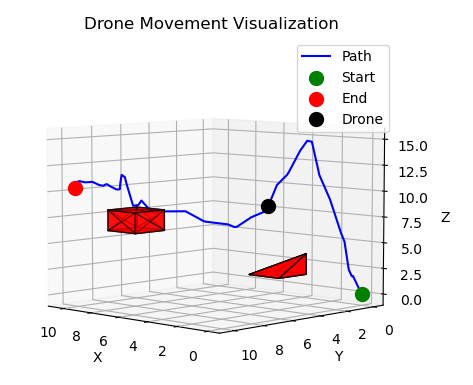
\includegraphics[width=0.7\linewidth]{fullDynamicPath.png}
\end{figure}

It took a long time to generate, like a few minutes and there were thousands of nodes.
A lot of controls and potential $q_{new}$ get thrown away for violating some of the states or for not being the closest to the sampled state.
The steps are also very small and when I play with the duration of the control it seems that a lot more controls and potential states get thrown out.
It seems that theres a very narrow window of legitimate controls to take you from one point towards another point.
I also have no idea how I could do path smoothing with this random control method, I would never get a random control that would take me on the new path.
There needs to be a better control design, I will continue to work on that but I don't think it will make it into this project submission


\section*{Drone Kinodynamics/home/steve0gillet/Downloads/AMP-report-style-file-master/AMP-report-style-file-master/AMP-report-style.sty}

\end{document}
